\chapter{Análisis de requisitos}\label{cap:analisis_de_requisitos}

Una vez contrastada la viabilidad de las ideas iniciales y analizadas las oportunidades del mercado, es imperativo \textbf{definir de manera precisa el comportamiento del sistema} antes de comenzar la fase de desarrollo técnico. Explicitar las funciones de negocio en este punto es un paso clave para construir un \textbf{producto robusto y libre de ambigüedades}. Con el fin de transformar de forma efectiva las aspiraciones generales plasmadas en los \hyperref[sec:objetivos_del_proyecto]{objetivos del proyecto}, la lógica de la aplicación se desglosa inicialmente en doce objetivos funcionales concretos que asientan las bases del sistema.

\begin{table}[H]
\centering
\small
\renewcommand{\arraystretch}{1.35}
\makebox[\textwidth][c]{%
\begin{tabularx}{1.1\textwidth}{l P{4cm} Y}
\bighline
\textbf{ID} & \textbf{Nombre} & \textbf{Descripción} \\ \bighline
OBJ-01\label{obj:01} & Módulo de usuario y autenticación & Proveer un sistema de autenticación seguro para profesores. \\ \hline
OBJ-02\label{obj:02} & Gestión de cuestionarios & Permitir la creación, edición y configuración de cuestionarios de preguntas. \\ \hline
OBJ-03\label{obj:03} & Creación de salas & Habilitar sesiones de test únicas identificadas mediante un código PIN. \\ \hline
OBJ-04\label{obj:04} & Acceso rápido & Permitir el acceso de alumnos a las salas mediante PIN y \textit{nickname} sin registro. \\ \hline
OBJ-05\label{obj:05} & Interacción en tiempo real & Sincronizar el estado de la partida y preguntas entre dispositivos. \\ \hline
OBJ-06\label{obj:06} & Verificación QR & Generar comprobante digital QR para validación presencial por el profesor. \\ \hline
OBJ-07\label{obj:07} & Persistencia validada & Almacenar en histórico solo los resultados verificados físicamente. \\ \hline 
OBJ-08\label{obj:08} & Estadísticas y análisis & Visualizar estadísticas de rendimiento basadas en datos validados. \\ \hline
OBJ-09\label{obj:09} & Asistente IA & Integrar IA para generar preguntas automáticamente según temáticas. \\ \hline
OBJ-10\label{obj:10} & Escaneo de código QR & Habilitar el uso de la cámara para la lectura ágil de códigos QR. \\ \hline
OBJ-11\label{obj:11} & Gestión de grupos & Organizar alumnos en clases para un seguimiento histórico. \\ \hline
OBJ-12\label{obj:12} & Exportación de datos & Permitir la descarga de resultados en formatos CSV/Excel. \\ \bighline
\end{tabularx}%
}
\caption{Objetivos funcionales de \textit{Quizzie}.}
\label{tab:objetivos_funcionales}
\end{table}

A lo largo de las siguientes secciones se identifican en primer lugar los actores que interactúan con la aplicación para, posteriormente, modelar su comportamiento mediante historias de usuario y casos de uso detallados. Asimismo, se determinan los requisitos de información, las reglas de negocio y los requisitos funcionales asociados a sus respectivos criterios de aceptación. El capítulo concluye con la definición de las restricciones no funcionales y la matriz de trazabilidad que garantiza la cobertura total del desarrollo propuesto.

\section{Historias de usuario}\label{sec:historias_de_usuario}

Una vez definidos los perfiles que interactúan con la plataforma, el comportamiento del sistema se define mediante historias de usuario siguiendo la metodología de elicitación de requisitos descrita por Sommerville \cite{sommerville2021engineering}. Estas especificaciones permiten capturar las necesidades reales de cada actor siguiendo la estructura clásica de rol \textbf{[como]}, acción \textbf{[quiero]} y beneficio \textbf{[para]}. Para facilitar la trazabilidad y el seguimiento de las historias, se han dividido y numerado de forma independiente según el perfil al que corresponden: el alumno (\textit{HU-AL}) y el profesor (\textit{HU-PR}).

\begin{table}[H]
\centering
\small
\renewcommand{\arraystretch}{1.35}
\makebox[\textwidth][c]{%
\begin{tabularx}{1.1\textwidth}{l l Y}
\bighline
\textbf{ID} & \textbf{Descripción} & \\ \bighline
HU-AL-01\label{hu:al-01} & \textbf{Como} alumno, & \textbf{quiero} unirme a una sala solo con un PIN y un apodo \\
                                  && \textbf{para} participar de forma inmediata sin necesidad de crear una cuenta. \\ \hline
HU-AL-02\label{hu:al-02} & \textbf{Como} alumno, & \textbf{quiero} recibir la pregunta y las opciones de respuesta en mi móvil de forma sincronizada \\
                                  && \textbf{para} competir en igualdad de condiciones con mis compañeros. \\ \hline
HU-AL-03\label{hu:al-03} & \textbf{Como} alumno, & \textbf{quiero} saber si mi respuesta ha sido correcta justo después de enviarla \\
                                  && \textbf{para} reforzar mi aprendizaje en el momento. \\ \hline
HU-AL-04\label{hu:al-04} & \textbf{Como} alumno, & \textbf{quiero} que se genere un código QR único al finalizar el test \\
                                  && \textbf{para} mostrárselo al profesor y que mi nota sea oficializada. \\ \hline
HU-AL-05\label{hu:al-05} & \textbf{Como} alumno, & \textbf{quiero} ver mi posición en el ranking después de cada bloque de preguntas \\
                                  && \textbf{para} motivarme durante la realización del cuestionario. \\ \hline
HU-AL-06\label{hu:al-06} & \textbf{Como} alumno, & \textbf{quiero} poder reengancharme a la partida si pierdo la conexión a internet \\
                                  && \textbf{para} no perder mi progreso y poder terminar el test. \\ \hline
HU-AL-07\label{hu:al-07} & \textbf{Como} alumno, & \textbf{quiero} recibir puntos extra por responder rápido o mantener una racha de aciertos \\
                                  && \textbf{para} sentirme recompensado por mi agilidad y constancia. \\ \bighline
\end{tabularx}%
}
\caption{Historias de usuario asociadas al rol de Alumno.}
\label{tab:hu_alumno}
\end{table}

\begin{table}[H]
\centering
\small
\renewcommand{\arraystretch}{1.35}
\makebox[\textwidth][c]{%
\begin{tabularx}{1.1\textwidth}{l l Y}
\bighline
\textbf{ID} & \textbf{Descripción} & \\ \bighline
HU-PR-01\label{hu:pr-01} & \textbf{Como} profesor, & \textbf{quiero} crear y organizar mis propios cuestionarios \\
                                  && \textbf{para} disponer de un repositorio de actividades personalizado por asignatura o tema. \\ \hline
HU-PR-02\label{hu:pr-02} & \textbf{Como} profesor, & \textbf{quiero} poder editar mis cuestionarios existentes \\
                                  && \textbf{para} corregir errores o crear variantes rápidas para diferentes grupos. \\ \hline
HU-PR-03\label{hu:pr-03} & \textbf{Como} profesor, & \textbf{quiero} crear y administrar una sala con un PIN único \\
                                  && \textbf{para} controlar el acceso de los alumnos y decidir cuándo comienza el test. \\ \hline
HU-PR-04\label{hu:pr-04} & \textbf{Como} profesor, & \textbf{quiero} ver en tiempo real qué están respondiendo los alumnos y quiénes se van conectando \\
                                  && \textbf{para} llevar un control del progreso de la clase. \\ \hline
HU-PR-05\label{hu:pr-05} & \textbf{Como} profesor, & \textbf{quiero} poder cerrar la sala una vez iniciada la actividad \\
                                  && \textbf{para} que ningún alumno se una tarde o de forma externa. \\ \hline
HU-PR-06\label{hu:pr-06} & \textbf{Como} profesor, & \textbf{quiero} escanear el móvil del alumno \\
                                  && \textbf{para} confirmar su presencia física y validar su nota en el sistema evitando respuestas no autorizadas. \\ \hline
HU-PR-07\label{hu:pr-07} & \textbf{Como} profesor, & \textbf{quiero} crear grupos o clases \\
                                  && \textbf{para} tener organizados a mis alumnos y facilitar el volcado de notas histórico. \\ \hline
HU-PR-08\label{hu:pr-08} & \textbf{Como} profesor, & \textbf{quiero} visualizar estadísticas de acierto por pregunta al finalizar \\
                                  && \textbf{para} detectar conceptos que no han quedado claros y reforzarlos. \\ \hline
HU-PR-09\label{hu:pr-09} & \textbf{Como} profesor, & \textbf{quiero} generar borradores de preguntas mediante IA \\
                                  && \textbf{para} reducir el tiempo de preparación de mis clases. \\ \hline
HU-PR-10\label{hu:pr-10} & \textbf{Como} profesor, & \textbf{quiero} exportar los resultados verificados a CSV \\
                                  && \textbf{para} integrarlos en mis herramientas de gestión docente externas. \\ \hline
HU-PR-11\label{hu:pr-11} & \textbf{Como} profesor, & \textbf{quiero} configurar si se otorgan puntos extra por rapidez o racha \\
                                  && \textbf{para} adaptar el nivel de competitividad de la sesión. \\ \hline
HU-PR-12\label{hu:pr-12} & \textbf{Como} profesor, & \textbf{quiero} decidir si el ranking se muestra tras cada pregunta \\
                                  && \textbf{para} gestionar el ritmo y la atención de la clase. \\ \hline
HU-PR-13\label{hu:pr-13} & \textbf{Como} profesor, & \textbf{quiero} añadir etiquetas e imágenes a mis cuestionarios \\
                                  && \textbf{para} identificarlos y personalizarlos visualmente. \\ \hline
HU-PR-14\label{hu:pr-14} & \textbf{Como} profesor, & \textbf{quiero} acceder al historial de salas pasadas \\
                                  && \textbf{para} revisar resultados y analizar el progreso de mis alumnos en el tiempo. \\ \bighline
\end{tabularx}%
}
\caption{Historias de usuario asociadas al rol de Profesor.}
\label{tab:hu_profesor}
\end{table}

\section{Reglas de negocio y restricciones}\label{sec:reglas_de_negocio_y_restricciones}

El correcto funcionamiento de la plataforma \textit{Quizzie} está sujeto a un conjunto de directrices operativas y limitaciones técnicas que garantizan tanto la validez funcional como la seguridad del sistema. 

\subsection{Reglas de negocio}\label{sec:reglas_de_negocio}

Las reglas de negocio definen las políticas, derechos y leyes lógicas que gobiernan el flujo de trabajo de la aplicación:

\begin{itemize}
    \item \textbf{Ciclo de vida de las salas:} Una sala de evaluación podrá encontrarse en espera, en juego, en fase de verificación o cerrada. Los alumnos carecerán de privilegios para alterar el estado operativo de la sesión.
    \item \textbf{Acceso a salas activas:} Un alumno solo podrá participar en una sala activa si introduce el código PIN correcto y un \textit{nickname} que no esté siendo utilizado por otro participante dentro de la misma sesión.
    \item \textbf{Validación presencial de calificaciones:} Ninguna calificación obtenida en una sesión en vivo se consolidará en el histórico permanente ni será válida para su exportación si no ha sido verificada físicamente en el aula mediante el escaneo del código QR del alumno por parte del dispositivo del profesor.
    \item \textbf{Caducidad y unicidad del token QR:} El código QR generado por el dispositivo del alumno al finalizar el test contendrá un token criptográfico único asociado a su sesión. Este token será de un solo uso; una vez escaneado y marcado como "Verificado", el sistema bloqueará cualquier intento posterior de lectura para evitar su duplicación.
    \item \textbf{Propiedad y gestión de cuestionarios:} Los cuestionarios creados, editados o eliminados lógicamente en la plataforma estarán asociados únicamente al profesor que los diseñó. Un docente no podrá visualizar, modificar ni utilizar para una sala los cuestionarios propiedad de otro usuario del sistema.
    \item \textbf{Generación asistida por IA:} El sistema proporcionará la generación automatizada de preguntas mediante Inteligencia Artificial, actuando como una herramienta de ayuda para el profesor. Todo contenido generado se considerará una propuesta preliminar, siendo responsabilidad exclusiva del profesor su revisión, edición y aprobación final.
    \item \textbf{Almacenamiento del historial de salas:} Una sala de evaluación se trasladará de forma definitiva al historial de sesiones pasadas únicamente tras concluir con éxito la fase de verificación presencial. En este registro permanente solo se consolidarán las calificaciones e identidades de aquellos alumnos que completaron el flujo de validación mediante código QR.
    \item \textbf{Análisis de rendimiento:} El sistema generará métricas analíticas orientadas a facilitar la detección de tendencias de aprendizaje en el aula, identificando automáticamente los conceptos con mayor índice de error y los patrones de acierto global del alumnado.
    \item \textbf{Exportación de resultados:} El profesorado dispondrá del derecho de portabilidad de las calificaciones oficiales del sistema, permitiendo la generación y descarga local de boletines de calificaciones en formatos estandarizados como PDF o CSV.
    \item \textbf{Seguimiento por grupos:} La plataforma permitirá la estructuración de los alumnos en grupos o clases con el fin de centralizar y evaluar la evolución histórica de un mismo conjunto de estudiantes a lo largo de diferentes sesiones académicas y cuestionarios.
\end{itemize}

\subsection{Restricciones}\label{sub:restricciones}
Para que las políticas de negocio descritas anteriormente puedan ejecutarse de manera efectiva, el sistema debe acatar una serie de restricciones técnicas y de diseño, aplicando el principio de arquitectura con autoridad en el servidor expuesto por Gregory \cite{gregory2014game}:

\begin{itemize}
    \item \textbf{Validación de \textit{uvus}:} El sistema restringirá el formato del \textit{uvus} de los alumnos para que coincida estrictamente con el patrón definido por la Universidad de Sevilla. El servidor validará mediante expresiones regulares que cumpla con los formatos oficiales, rechazando cualquier formato de nombre inválido.
    \item \textbf{Dimensionamiento de cuestionarios:} En la creación de contenido se impondrá un límite estructural rígido por motivos de maquetación de la interfaz móvil y rendimiento de la base de datos, restringiendo cada cuestionario a un máximo de 30 preguntas y fijando un límite máximo de 8 opciones de respuesta por cada enunciado.
    \item \textbf{Persistencia ante desconexiones:} Ante una pérdida accidental de conectividad a internet por parte de un alumno en plena partida, el backend retendrá su estado y puntuación. Esto permitirá su reconexión mientras la sala siga activa sin perder las respuestas previas a la desconexión.
    \item \textbf{Protocolos de comunicación síncrona:} Para garantizar la sincronización en tiempo real y asegurar que los eventos de la partida se procesen con la latencia mínima requerida, la comunicación bidireccional entre los dispositivos de la sala (profesor/alumnos) estará restringida exclusivamente al uso del protocolo seguro \textit{WebSockets} (\texttt{WSS}).
    \item \textbf{Cifrado de credenciales:} El sistema operativo del backend prohibirá el almacenamiento de contraseñas en texto plano dentro de la base de datos. Será obligatorio aplicar un algoritmo de \textit{hashing} seguro y unidireccional antes de cualquier operación de persistencia de credenciales de profesores.
    \item \textbf{Seguridad del código QR:} El \textit{token} incrustado en el código QR del alumno deberá generarse mediante criptografía segura y no falsificable desde el servidor. 
\end{itemize}

\section{Requisitos de información}\label{sec:requisitos_de_informacion}

Los requisitos de información determinan los conjuntos de datos que el sistema debe almacenar de forma persistente para garantizar el correcto funcionamiento de la aplicación y dar soporte a las reglas de negocio e historias de usuario definidas. En esta fase de análisis no se busca detallar la estructura técnica de las tablas, las restricciones de integridad ni sus atributos específicos. Dichos aspectos se detallarán en el capítulo dedicado a \hyperref[cap:diseno_y_arquitectura]{Diseño y arquitectura}.

\begin{table}[H]
\centering
\small
\renewcommand{\arraystretch}{1.35}
\makebox[\textwidth][c]{%
\begin{tabularx}{1.06\textwidth}{l P{3.3cm} Y}
\bighline
\textbf{ID} & \textbf{Nombre} & \textbf{Descripción} \\ \bighline
RI-01\label{ri:01} & Profesores y cuentas & Credenciales de acceso de los profesores (correo electrónico y el \textit{hash} de la contraseña) y su nombre visible. \\ \hline
RI-02\label{ri:02} & Cuestionarios y preguntas & Datos relativos a los tests diseñados por los profesores. Incluye los campos básicos del cuestionario (título, descripción) y la composición de sus preguntas y opciones asociadas. \\ \hline
RI-03\label{ri:03} & Configuración y control de salas & Código PIN único de acceso, el estado operativo de la sala (espera, en juego, en fase de verificación o cerrada), el temporizador del servidor para la sincronización mediante \textit{WebSockets}. \\ \hline
RI-04\label{ri:04} & Registro temporal de participación & Datos de alumnos conectados identificados mediante su \textit{uvus}, opciones seleccionadas y puntuaciones obtenidas. \\ \hline
RI-05\label{ri:05} & Comprobantes de presencialidad y tokens QR & Validación de notas y mitigación del fraude digital. Debe almacenar el token criptográfico seguro y firmado digitalmente que se asocia a cada alumno al terminar un test, su estado de verificación actual. \\ \hline
RI-06\label{ri:06} & Histórico de calificaciones y respuestas & Salas que han completado con éxito la fase de verificación presencial. Debe registrar los mismos datos de cada alumno que el registro temporal, pero con el estado de verificación completado y persistiendo dichos datos. \\ \hline
RI-07\label{ri:07} & Gestión de grupos & Etiquetas de grupo o clase, profesor responsable y lista de alumnos asociados. \\ \bighline
\end{tabularx}%
}
\caption{Requisitos de información.}
\label{tab:requisitos_informacion}
\end{table}

\section{Requisitos funcionales}\label{sec:requisitos_funcionales}

Los requisitos funcionales determinan las acciones específicas, comportamientos y servicios que la plataforma \textit{Quizzie} debe ejecutar para satisfacer las necesidades de los usuarios. Este catálogo traduce las historias de usuario y las políticas lógicas del sistema en directrices operativas de desarrollo. A continuación, se detallan los requisitos funcionales del sistema:

\begin{table}[H]
\centering
\small
\renewcommand{\arraystretch}{1.35}
\makebox[\textwidth][c]{%
\begin{tabularx}{1.1\textwidth}{l P{2.4cm} Y c}
\bighline
\textbf{ID} & \textbf{Nombre} & \textbf{Descripción} & \textbf{Prioridad} \\ \bighline
RF-01\label{req:01} & Gestión de registro & Registro de nuevos profesores con validación de correo electrónico y \textit{hash} de contraseña. & \covRed{Alta} \\ \hline
RF-02\label{req:02} & Inicio de sesión & Autenticación de docentes mediante correo electrónico y contraseña cifrada con emisión de tokens JWT. & \covRed{Alta} \\ \hline
RF-03\label{req:03} & Baja de usuarios & Eliminación de la cuenta de profesor y todos sus datos asociados de forma permanente del sistema. & \covYellow{Media} \\ \hline
RF-04\label{req:04} & Recuperación contraseña & Solicitud y tramitación de restablecimiento de credenciales de acceso vía correo electrónico. & \covGreen{Baja} \\ \hline
RF-05\label{req:05} & Edición perfil & Modificación de los datos de usuario del profesor, incluyendo el nombre visible y la contraseña. & \covYellow{Media} \\ \hline
RF-06\label{req:06} & Cierre de sesión & Invalidación del token de autenticación activo en el servidor y redirección automática al formulario de acceso. & \covRed{Alta} \\ \hline
RF-07\label{req:07} & Crear cuestionario & Creación de nuevas pruebas de evaluación con un límite máximo estructurado de hasta 30 preguntas. & \covRed{Alta} \\ \hline
RF-08\label{req:08} & Listar cuestionarios & Visualización del catálogo de pruebas diseñadas por el profesor, ordenadas cronológicamente por fecha. & \covRed{Alta} \\ \hline
RF-09\label{req:09} & Mostrar ranking & Presentación de la tabla de clasificación de alumnos después de cada pregunta y al finalizar la sesión. & \covYellow{Media} \\ \hline
RF-10\label{req:10} & Aleatoriedad & Configuración opcional para alterar de forma automática el orden de las preguntas y sus respectivas respuestas. & \covGreen{Baja} \\ \hline
RF-11\label{req:11} & Configurar tiempo & Definición personalizada del tiempo límite de respuesta para cada enunciado durante la creación de la sala. & \covYellow{Media} \\ \hline
RF-12\label{req:12} & Importación & Carga de preguntas y opciones desde archivos externos estructurados exclusivamente en formato \texttt{.txt} o \texttt{.csv}. & \covYellow{Media} \\ \hline
RF-13\label{req:13} & Edición de cuestionarios & Modificación integral del título, descripción, enunciados y opciones de respuestas de un test existente. & \covYellow{Media} \\ \hline
RF-14\label{req:14} & Eliminación de datos & Borrado lógico en el sistema de cuestionarios o preguntas individuales sin destruir el histórico pasado. & \covYellow{Media} \\ \hline
RF-15\label{req:15} & Crear sala & Instanciación en tiempo real de una sesión de evaluación protegida mediante un código PIN único de acceso. & \covRed{Alta} \\ \hline
RF-16\label{req:16} & Validar PIN & Verificación inmediata en el servidor de que el código PIN introducido corresponde a una sala en estado de espera. & \covRed{Alta} \\ \hline
RF-17\label{req:17} & Validar \textit{uvus} & Control de acceso que valida el formato alfanumérico institucional de la Universidad de Sevilla y mitiga duplicados. & \covRed{Alta} \\ \hline
RF-18\label{req:18} & Sala de espera & Gestión y mantenimiento del flujo de alumnos conectados en tiempo real mediante \textit{WebSockets} antes del inicio. & \covRed{Alta} \\ \hline
RF-19\label{req:19} & Cerrar sala & Finalización manual o automática de la sesión, despliegue de resultados finales y desconexión de los participantes. & \covYellow{Media} \\ \bighline
\end{tabularx}%
}
\caption{Requisitos funcionales (del RF-01 al RF-19).}
\label{tab:requisitos_funcionales_1}
\end{table}

\begin{table}[H]
\centering
\small
\renewcommand{\arraystretch}{1.35}
\makebox[\textwidth][c]{%
\begin{tabularx}{1.1\textwidth}{l P{2.4cm} Y c}
\bighline
\textbf{ID} & \textbf{Nombre} & \textbf{Descripción} & \textbf{Prioridad} \\ \bighline
RF-20\label{req:20} & Comenzar sala & Activación de la cuenta atrás sincronizada en el servidor y apertura de la primera pregunta del test. & \covRed{Alta} \\ \hline
RF-21\label{req:21} & Distribución síncrona & Envío simultáneo de la secuencia de enunciados y opciones desde el backend a todos los clientes conectados. & \covRed{Alta} \\ \hline
RF-22\label{req:22} & Temporizador servidor & Control centralizado y ejecución estricta del tiempo de respuesta remota en el hilo del backend. & \covRed{Alta} \\ \hline
RF-23\label{req:23} & Recepción respuestas & Captura, marca de tiempo y procesamiento de la opción de respuesta seleccionada por el alumno. & \covRed{Alta} \\ \hline
RF-24\label{req:24} & Feedback inmediato & Notificación instantánea en el dispositivo del alumno sobre el acierto o fallo sin consolidar la nota permanente. & \covRed{Alta} \\ \hline
RF-25\label{req:25} & Registro provisional & Almacenamiento transitorio del resultado del participante bajo el estado de "No Verificado" y emisión de un token único. & \covRed{Alta} \\ \hline
RF-26\label{req:26} & Generación QR & Renderizado de un código QR dinámico en la pantalla del alumno que encapsula su identidad y su token criptográfico. & \covRed{Alta} \\ \hline
RF-27\label{req:27} & Activación cámara & Solicitud de permisos e inicialización del flujo de vídeo de la cámara web en el dispositivo del profesor. & \covRed{Alta} \\ \hline
RF-28\label{req:28} & Lectura de QR & Captura óptica, decodificación y extracción de la estructura de datos del alumno desde la interfaz docente. & \covRed{Alta} \\ \hline
RF-29\label{req:29} & Validación Token & Comparación criptográfica en el servidor del token escaneado frente al registro transitorio de la sesión activa. & \covRed{Alta} \\ \hline
RF-30\label{req:30} & Control de estado & Bloqueo lógico automático de solicitudes de validación de notas si el registro ya consta como "Verificado". & \covRed{Alta} \\ \hline
RF-31\label{req:31} & Check verificación & Actualización de la sesión a estado verificado y consolidación oficial de la nota en el histórico definitivo. & \covRed{Alta} \\ \hline
RF-32\label{req:32} & Listado en vivo & Actualización en tiempo real del panel docente reflejando la lista de alumnos validados presencialmente. & \covYellow{Media} \\ \hline
RF-33\label{req:33} & Estadísticas de sala & Cálculo de los porcentajes de acierto y fallo por enunciado para la detección automatizada de conceptos complejos. & \covYellow{Media} \\ \hline
RF-34\label{req:34} & Generación por IA & Procesamiento automatizado de textos introducidos por el docente para la sugerencia de borradores de preguntas mediante IA. & \covYellow{Media} \\ \hline
RF-35\label{req:35} & Asistente de ayuda & Resolución de dudas conceptuales y de uso del sistema mediante una interfaz de lenguaje natural integrada. & \covGreen{Baja} \\ \hline
RF-36\label{req:36} & Navegación por IA & Sistema de soporte inteligente encargado de detectar intenciones de uso y guiar al profesor en el entorno web. & \covGreen{Baja} \\ \hline
RF-37\label{req:37} & Revisión post IA & Interfaz de edición específica para la inspección manual, corrección y aprobación de las preguntas sugeridas por la IA. & \covYellow{Media} \\ \bighline
\end{tabularx}%
}
\caption{Requisitos funcionales (del RF-20 al RF-37).}
\label{tab:requisitos_funcionales_2}
\end{table}

\begin{table}[H]
\centering
\small
\renewcommand{\arraystretch}{1.35}
\makebox[\textwidth][c]{%
\begin{tabularx}{1.1\textwidth}{l P{2.4cm} Y c}
\bighline
\textbf{ID} & \textbf{Nombre} & \textbf{Descripción} & \textbf{Prioridad} \\ \bighline
RF-38\label{req:38} & Crear clase & Agrupación e indexación de conjuntos estables de alumnos bajo etiquetas de grupo o clase académica. & \covGreen{Baja} \\ \hline
RF-39\label{req:39} & Exportación resultados & Generación y descarga local de las calificaciones oficiales y verificadas en formatos estandarizados PDF o CSV. & \covRed{Alta} \\ \hline
RF-40\label{req:40} & Gestión de conexiones & Manejo de admisiones tardías, retención de estados por caída de red y flujos de reconexión adaptativa. & \covYellow{Media} \\ \hline
RF-41\label{req:41} & Filtros de búsqueda & Herramientas de filtrado avanzado en el catálogo de cuestionarios (activos, inactivos, recientes o etiquetas). & \covYellow{Media} \\ \hline
RF-42\label{req:42} & Bonificación por tiempo & Algoritmo de cálculo de puntuación adicional ponderada según la rapidez de respuesta del participante. & \covGreen{Baja} \\ \hline
RF-43\label{req:43} & Sistema de rachas & Concesión de multiplicadores de puntuación por el encadenamiento consecutivo de respuestas correctas. & \covGreen{Baja} \\ \hline
RF-44\label{req:44} & Modo de puntuación & Selección de las reglas de asignación de puntos (estándar o adaptativa) en los parámetros iniciales de la sala. & \covGreen{Baja} \\ \hline
RF-45\label{req:45} & Visibilidad de ranking & Opción para conmutar la presencia de la pantalla intermedia de clasificación global entre preguntas. & \covGreen{Baja} \\ \hline
RF-46\label{req:46} & Formulario avanzado & Inclusión de imágenes de soporte y gestión de etiquetas avanzadas (tags) en la edición del cuestionario. & \covGreen{Baja} \\ \hline
RF-47\label{req:47} & Historial de salas & Acceso permanente al registro histórico de sesiones cerradas que hayan completado la fase de verificación presencial. & \covRed{Alta} \\ \bighline
\end{tabularx}%
}
\caption{Requisitos funcionales (del RF-38 al RF-47).}
\label{tab:requisitos_funcionales_3}
\end{table}

\subsection{Criterios de aceptación y definición de hecho}\label{sub:criterios_de_aceptacion}

Para garantizar que los requisitos funcionales especificados alcancen los estándares de calidad, seguridad y robustez técnica exigidos, el proceso de desarrollo se rige por una \textbf{\textit{Definition of Done}} (\textbf{DoD}). Este marco actúa como una lista de comprobación obligatoria y transversal que cualquier funcionalidad debe satisfacer antes de ser dada por finalizada y consolidada en el sistema.

De manera general, un requisito funcional se considerará formalmente aceptado cuando cumpla con las siguientes dimensiones de verificación:

\begin{itemize}
    \item \textbf{Comportamiento funcional:}
    \begin{itemize}
        \item \textbf{Flujo principal:} Se ejecuta correctamente en la interfaz del usuario sin producir bloqueos, errores ni excepciones no controladas.
        \item \textbf{Gestión de excepciones:} El sistema gestiona los flujos alternativos y de error (entradas inválidas, caídas de red o datos duplicados) devolviendo un \textit{feedback} informativo e inmediato al usuario.
        \item \textbf{Restricciones operativas:} Se respetan los límites físicos, lógicos y de formato estructurados en las reglas de negocio y restricciones del sistema.
    \end{itemize}

    \item \textbf{Calidad técnica y seguridad:}
    \begin{itemize}
        \item \textbf{Seguridad de datos:} El código fuente cumple con las directrices relativas a la persistencia íntegra de la información y al cifrado estricto de credenciales.
        \item \textbf{Protocolos de red:} Las comunicaciones síncronas o en tiempo real emplean de forma estricta los canales bidireccionales y protocolos establecidos en la arquitectura.
        \item \textbf{Integridad del modelo:} Los datos asociados se mapean de forma exacta en las estructuras definidas en los requisitos de información.
    \end{itemize}

    \item \textbf{Verificación y pruebas:}
    \begin{itemize}
        \item \textbf{Cobertura de pruebas:} La funcionalidad tiene asociado, al menos, un caso de prueba unitario, de integración o de sistema dentro del plan de verificación.
        \item \textbf{Validación de resultados:} El comportamiento real del software coincide con el esperado tras superar con éxito las pruebas funcionales, de carga o de seguridad.
    \end{itemize}

    \item \textbf{Documentación y gestión del ciclo de vida:}
    \begin{itemize}
        \item \textbf{Mantenibilidad:} Se ha redactado la documentación técnica correspondiente en los módulos afectados, incluyendo tipado estricto y comentarios según las buenas prácticas de desarrollo.
        \item \textbf{Trazabilidad en control de versiones:} El \textit{issue} asignado en GitHub se ha actualizado con la solución implementada, asociando los \textit{commits} pertinentes y procediendo a su cierre formal tras la aprobación del despliegue.
    \end{itemize}
\end{itemize}

Estos criterios globales de aceptación aseguran que el paso del análisis de requisitos a la fase de pruebas finales sea completamente \textbf{trazable, transparente y verificable}, sirviendo de base para la posterior verificación del sistema en la sección dedicada a los \hyperref[sec:casos_de_prueba_y_validacion]{casos de prueba y su validación}.

\section{Casos de uso}\label{sec:casos_de_uso}

Los diagramas y especificaciones de casos de uso sirven para modelar el comportamiento del sistema desde el punto de vista de los actores involucrados, transformando los requisitos funcionales abstractos en interacciones lógicas concretas. Con el propósito de mantener la claridad de la memoria y evitar redundancias estructurales, las funcionalidades de la plataforma \textit{Quizzie} se estructuran en paquetes funcionales según el área operativa donde actúan los usuarios principales (\textit{Profesor} y \textit{Alumno}).

\begin{figure}[H]
    \centering
    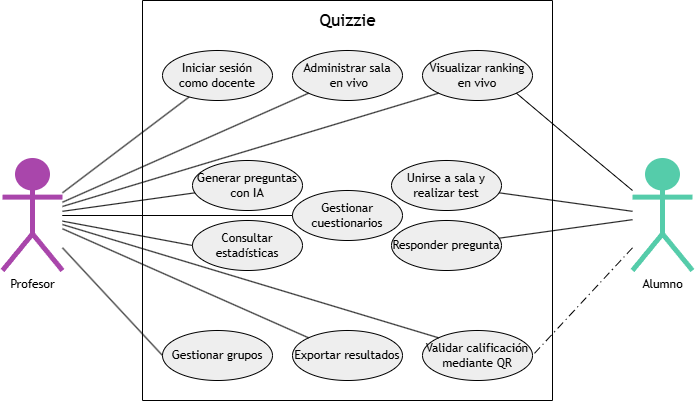
\includegraphics[width=0.95\textwidth]{figures/casos_de_uso.png}
    \vspace{0.5cm}
    \caption{Diagrama general de casos de uso del sistema.}
    \label{fig:diagrama_casos_uso}
\end{figure}

El conjunto de los casos de uso que componen el sistema es el siguiente:

\begin{itemize}
    \item \textbf{CU-01: Iniciar sesión como docente.} Permite al profesor acceder a su panel privado, registrarse o cerrar sesión de forma segura.
    \item \textbf{CU-02: Gestionar cuestionarios.} El profesor puede crear, editar, listar y eliminar sus bancos de preguntas.
    \item \textbf{CU-03: Generar preguntas con IA.} Extensión del CU-02 donde el profesor solicita a la IA la creación de borradores de preguntas basados en un tema.
    \item \textbf{CU-04: Administrar sala en vivo.} El profesor instancia un cuestionario, genera un PIN de acceso y controla el flujo de la partida (inicio, paso de preguntas y cierre).
    \item \textbf{CU-05: Unirse a sala y realizar test.} El alumno accede mediante PIN, responde a las preguntas sincronizadas y recibe feedback inmediato sobre su rendimiento.
    \item \textbf{CU-06: Visualizar ranking en vivo.} Los alumnos y el profesor visualizan la progresión de los líderes de la sala tras cada pregunta.
    \item \textbf{CU-07: Validar calificación mediante QR.} El profesor utiliza su dispositivo para escanear el código QR del alumno, verificando su identidad y presencia física para oficializar la calificación.
    \item \textbf{CU-08: Consultar estadísticas.} El profesor analiza los puntos críticos y el rendimiento general de la clase tras finalizar la sesión.
    \item \textbf{CU-09: Exportar resultados.} El profesor descarga los datos de los alumnos verificados en formato CSV para su uso en plataformas externas.
    \item \textbf{CU-10: Responder pregunta.} El alumno puede responder durante el tiempo determinado a las preguntas del test obteniendo la puntuación pertinente.
    \item \textbf{CU-11: Gestionar grupos.} El profesor organiza el alumnado creando etiquetas de grupo para asociar y evaluar la evolución histórica de un mismo conjunto de estudiantes.
\end{itemize}

\subsection{Especificación detallada de Casos de Uso}\label{sub:especificacion_casos_de_uso}

A continuación, se detallan las plantillas descriptivas de cada caso de uso del sistema, especificando sus actores, precondiciones, secuencias de pasos lógicos y la gestión de escenarios alternativos de error:

\begin{table}[H]
\centering
\small
\renewcommand{\arraystretch}{1.3}
\setlength{\tabcolsep}{6pt}
\makebox[\textwidth][c]{%
\begin{tabularx}{1.1\textwidth}{l Y}
\bighline
\multicolumn{2}{c}{\textbf{CU-01: Iniciar sesión como docente}\label{cu:01}} \\ \bighline
\textbf{Actor principal} & Profesor. \\ \hline
\textbf{Precondición} & El profesor debe estar registrado en la plataforma. \\ \hline
\textbf{Flujo principal} & 1. El profesor introduce su correo electrónico y contraseña en el formulario de login. \\ \cline{2-2}
                         & 2. El sistema cifra la contraseña introducida y la compara con el \textit{hash} almacenado. \\ \cline{2-2}
                         & 3. El sistema genera un token de sesión (JWT) y redirige al profesor a su panel principal. \\ \hline
\textbf{Flujo alternativo} & Si las credenciales son incorrectas, el sistema muestra un mensaje de error y permite reintentar el acceso. \\ \bighline
\end{tabularx}%
}
\caption[CU-01: Iniciar sesión como docente]{Especificación del caso de uso CU-01.}
\label{tab:cu_01}
\end{table}

\vfill

\begin{table}[H]
\centering
\small
\renewcommand{\arraystretch}{1.3}
\setlength{\tabcolsep}{6pt}
\makebox[\textwidth][c]{%
\begin{tabularx}{1.1\textwidth}{l Y}
\bighline
\multicolumn{2}{c}{\textbf{CU-02: Gestionar cuestionarios}\label{cu:02}} \\ \bighline
\textbf{Actor principal} & Profesor. \\ \hline
\textbf{Precondición} & El profesor ha iniciado sesión correctamente. \\ \hline
\textbf{Flujo principal} & 1. El profesor accede a su biblioteca de contenidos. \\ \cline{2-2}
                         & 2. Selecciona la opción de crear un nuevo cuestionario o editar uno existente. \\ \cline{2-2}
                         & 3. El profesor define el título, descripción y añade preguntas con sus respectivas opciones. \\ \cline{2-2}
                         & 4. El profesor marca la opción correcta para cada pregunta y asigna una puntuación. \\ \cline{2-2}
                         & 5. El sistema guarda los cambios en la base de datos permanente. \\ \hline
\textbf{Postcondición} & El cuestionario queda disponible para ser utilizado en una sala. \\ \bighline
\end{tabularx}%
}
\caption[CU-02: Gestionar cuestionarios]{Especificación del caso de uso CU-02.}
\label{tab:cu_02}
\end{table}

\newpage

\begin{table}[H]
\centering
\small
\renewcommand{\arraystretch}{1.2}
\setlength{\tabcolsep}{6pt}
\makebox[\textwidth][c]{%
\begin{tabularx}{1.1\textwidth}{l Y}
\bighline
\multicolumn{2}{c}{\textbf{CU-03: Generar preguntas con IA}\label{cu:03}} \\ \bighline
\textbf{Actores} & Principal: Profesor. Secundario: Servicio de IA (API). \\ \hline
\textbf{Precondición} & El profesor se encuentra dentro del editor de cuestionarios. \\ \hline
\textbf{Flujo principal} & 1. El profesor activa el asistente de IA e introduce un tema o pega un texto base. \\ \cline{2-2}
                         & 2. El sistema envía la información a la API de IA externa. \\ \cline{2-2}
                         & 3. El sistema recibe y presenta al profesor un listado de preguntas y respuestas sugeridas. \\ \cline{2-2}
                         & 4. El profesor selecciona las preguntas que desea importar y las edita si es necesario. \\ \cline{2-2}
                         & 5. El sistema integra las preguntas seleccionadas en el cuestionario actual. \\ \bighline
\end{tabularx}%
}
\caption[CU-03: Generar preguntas con IA]{Especificación del caso de uso CU-03.}\label{tab:cu_03}
\end{table}

\vfill

\begin{table}[H]
\centering
\small
\renewcommand{\arraystretch}{1.2}
\setlength{\tabcolsep}{6pt}
\makebox[\textwidth][c]{%
\begin{tabularx}{1.1\textwidth}{l Y}
\bighline
\multicolumn{2}{c}{\textbf{CU-04: Administrar sala en vivo}\label{cu:04}} \\ \bighline
\textbf{Actor principal} & Profesor. \\ \hline
\textbf{Precondición} & El profesor está autenticado y ha seleccionado un cuestionario de su biblioteca. \\ \hline
\textbf{Flujo principal} & 1. El profesor solicita la creación de una nueva sala de juego. \\ \cline{2-2}
                         & 2. El sistema genera un PIN único de 6 dígitos y abre el \textit{socket} de comunicación. \\ \cline{2-2}
                         & 3. El profesor controla en tiempo real la entrada de alumnos en la sala de espera. \\ \cline{2-2}
                         & 4. El profesor inicia el test, enviando la señal de comienzo a todos los alumnos. \\ \cline{2-2}
                         & 5. El profesor controla el paso de las preguntas o permite el avance automático. \\ \cline{2-2}
                         & 6. El profesor finaliza la sesión manualmente o al terminar las preguntas. \\ \bighline
\end{tabularx}%
}
\caption[CU-04: Administrar sala en vivo]{Especificación del caso de uso CU-04.}\label{tab:cu_04}
\end{table}

\vfill

\begin{table}[H]
\centering
\small
\renewcommand{\arraystretch}{1.2}
\setlength{\tabcolsep}{6pt}
\makebox[\textwidth][c]{%
\begin{tabularx}{1.1\textwidth}{l Y}
\bighline
\multicolumn{2}{c}{\textbf{CU-05: Unirse a sala y realizar test}\label{cu:05}} \\ \bighline
\textbf{Actor principal} & Alumno. \\ \hline
\textbf{Precondición} & Existe una sala activa y el alumno posee el código PIN. \\ \hline
\textbf{Flujo principal} & 1. El alumno introduce el PIN y un \textit{nickname}. \\ \cline{2-2}
                         & 2. El sistema valida el acceso y posiciona al alumno en la sala de espera. \\ \cline{2-2}
                         & 3. Al comenzar el test, el alumno recibe las preguntas de forma sincronizada con el resto de la clase. \\ \cline{2-2}
                         & 4. El alumno selecciona la opción deseada dentro del tiempo límite. \\ \cline{2-2}
                         & 5. El sistema registra la respuesta y el tiempo empleado. \\ \cline{2-2}
                         & 6. Al finalizar el \textit{quiz}, el alumno recibe un código QR único de validación. \\ \hline
\textbf{Flujo alternativo} & Si el alumno sufre una desconexión, puede reingresar con el mismo PIN y \textit{nickname}; el sistema restaurará su sesión y lo situará en la pregunta activa. \\ \bighline
\end{tabularx}%
}
\caption[CU-05: Unirse a sala y realizar test]{Especificación del caso de uso CU-05.}
\label{tab:cu_05}
\end{table}

\newpage

\begin{table}[H]
\centering
\small
\renewcommand{\arraystretch}{1.25}
\setlength{\tabcolsep}{6pt}
\makebox[\textwidth][c]{%
\begin{tabularx}{1.1\textwidth}{l Y}
\bighline
\multicolumn{2}{c}{\textbf{CU-06: Visualizar ranking en vivo}\label{cu:06}} \\ \bighline
\textbf{Actores} & Principal: Profesor / Alumno. \\ \hline
\textbf{Precondición} & Se ha completado al menos una pregunta en una sala activa. \\ \hline
\textbf{Flujo principal} & 1. El sistema calcula la puntuación de cada alumno basándose en aciertos y velocidad de respuesta. \\ \cline{2-2}
                         & 2. El sistema actualiza el ranking global de la sala. \\ \cline{2-2}
                         & 3. El profesor visualiza el ``Top 5'' en la pantalla principal para motivar a la clase. \\ \cline{2-2}
                         & 4. El alumno visualiza su posición relativa y sus puntos en su propio dispositivo. \\ \bighline
\end{tabularx}%
}
\caption[CU-06: Visualizar ranking en vivo]{Especificación del caso de uso CU-06.}
\label{tab:cu_06}
\end{table}

\vfill

\begin{table}[H]
\centering
\small
\renewcommand{\arraystretch}{1.25}
\setlength{\tabcolsep}{6pt}
\makebox[\textwidth][c]{%
\begin{tabularx}{1.1\textwidth}{l Y}
\bighline
\multicolumn{2}{c}{\textbf{CU-07: Validar calificación mediante QR}\label{cu:07}} \\ \bighline
\textbf{Actores} & Principal: Profesor. Secundario: Alumno. \\ \hline
\textbf{Precondición} & La sala ha finalizado y el alumno muestra el QR generado por el sistema. \\ \hline
\textbf{Flujo principal} & 1. El profesor selecciona la opción de ``Validar Alumno'' en su panel de sala. \\ \cline{2-2}
                         & 2. El profesor escanea el código QR del dispositivo del alumno. \\ \cline{2-2}
                         & 3. El sistema extrae el token cifrado del QR y lo valida contra el registro provisional en el backend. \\ \cline{2-2}
                         & 4. Tras la validación positiva, el sistema cambia el estado del alumno a ``Verificado''. \\ \cline{2-2}
                         & 5. La nota se hace persistente y se vincula oficialmente al registro del alumno. \\ \bighline
\end{tabularx}%
}
\caption[CU-07: Validar calificación mediante QR]{Especificación del caso de uso CU-07.}
\label{tab:cu_07}
\end{table}

\vfill

\begin{table}[H]
\centering
\small
\renewcommand{\arraystretch}{1.25}
\setlength{\tabcolsep}{6pt}
\makebox[\textwidth][c]{%
\begin{tabularx}{1.1\textwidth}{l Y}
\bighline
\multicolumn{2}{c}{\textbf{CU-08: Consultar estadísticas}\label{cu:08}} \\ \bighline
\textbf{Actor principal} & Profesor. \\ \hline
\textbf{Precondición} & Existen salas finalizadas con respuestas registradas. \\ \hline
\textbf{Flujo principal} & 1. El profesor accede al histórico de salas desde su panel. \\ \cline{2-2}
                         & 2. Selecciona una sesión específica para analizar. \\ \cline{2-2}
                         & 3. El sistema genera gráficas comparativas sobre el porcentaje de aciertos por pregunta. \\ \cline{2-2}
                         & 4. El profesor identifica las áreas de conocimiento donde los alumnos han tenido más dificultades. \\ \bighline
\end{tabularx}%
}
\caption[CU-08: Consultar estadísticas]{Especificación del caso de uso CU-08.}
\label{tab:cu_08}
\end{table}

\newpage

\begin{table}[H]
\centering
\small
\renewcommand{\arraystretch}{1.2}
\setlength{\tabcolsep}{6pt}
\makebox[\textwidth][c]{%
\begin{tabularx}{1.1\textwidth}{l Y}
\bighline
\multicolumn{2}{c}{\textbf{CU-09: Exportar resultados}\label{cu:09}} \\ \bighline
\textbf{Actor principal} & Profesor. \\ \hline
\textbf{Precondición} & La sala ha finalizado y existen alumnos con estado ``Verificado''. \\ \hline
\textbf{Flujo principal} & 1. El profesor solicita la exportación de resultados desde el informe de la sala. \\ \cline{2-2}
                         & 2. El sistema filtra los datos para incluir únicamente los resultados verificados. \\ \cline{2-2}
                         & 3. El sistema genera un archivo en formato CSV o Excel. \\ \cline{2-2}
                         & 4. El archivo se descarga automáticamente en el dispositivo del profesor. \\ \bighline
\end{tabularx}%
}
\caption[CU-09: Exportar resultados]{Especificación del caso de uso CU-09.}
\label{tab:cu_09}
\end{table}

\begin{table}[H]
\centering
\small
\renewcommand{\arraystretch}{1.2}
\setlength{\tabcolsep}{6pt}
\makebox[\textwidth][c]{%
\begin{tabularx}{1.1\textwidth}{l Y}
\bighline
\multicolumn{2}{c}{\textbf{CU-10: Responder pregunta}\label{cu:10}} \\ \bighline
\textbf{Actor principal} & Alumno. \\ \hline
\textbf{Precondición} & El alumno está en una sala activa y el profesor ha lanzado una pregunta. \\ \hline
\textbf{Flujo principal} & 1. El sistema muestra el enunciado y las opciones de respuesta en el dispositivo del alumno. \\ \cline{2-2}
                         & 2. El sistema inicia el cronómetro de cuenta atrás definido para esa sala. \\ \cline{2-2}
                         & 3. El alumno selecciona una de las opciones antes de que el tiempo se agote. \\ \cline{2-2}
                         & 4. El sistema captura la opción elegida y el tiempo de la respuesta (\textit{timestamp}). \\ \cline{2-2}
                         & 5. Al agotarse el tiempo o responder todos los alumnos, el sistema cierra la recepción de datos. \\ \cline{2-2}
                         & 6. El sistema mira si la respuesta es correcta y calcula los puntos obtenidos. \\ \hline
\textbf{Flujo alternativo} & Si el alumno no selecciona ninguna opción antes de que el cronómetro llegue a cero, el sistema registra la pregunta como ``No contestada'' con 0 puntos. \\ \hline
\textbf{Postcondición} & El resultado de la pregunta se almacena temporalmente para actualizar el ranking en vivo. \\ \bighline
\end{tabularx}%
}
\caption[CU-10: Responder pregunta]{Especificación del caso de uso CU-10.}
\label{tab:cu_10}
\end{table}

\begin{table}[H]
\centering
\small
\renewcommand{\arraystretch}{1.2}
\setlength{\tabcolsep}{6pt}
\makebox[\textwidth][c]{%
\begin{tabularx}{1.1\textwidth}{l Y}
\bighline
\multicolumn{2}{c}{\textbf{CU-11: Gestionar grupos}\label{cu:11}} \\ \bighline
\textbf{Actor principal} & Profesor. \\ \hline
\textbf{Precondición} & El profesor ha iniciado sesión correctamente en el sistema. \\ \hline
\textbf{Flujo principal} & 1. El profesor accede a la sección de gestión de grupos desde el panel de control. \\ \cline{2-2}
                         & 2. Selecciona la opción de crear una nueva clase e introduce un nombre descriptivo o etiqueta de grupo. \\ \cline{2-2}
                         & 3. El profesor asocia la lista de identificadores de alumnos válidos correspondientes a ese conjunto académico. \\ \cline{2-2}
                         & 4. El sistema almacena la estructura del grupo vinculándola directamente al perfil del docente responsable. \\ \cline{2-2}
                         & 5. El profesor consulta los reportes específicos para comprobar el progreso y la evolución histórica de las calificaciones de dicha clase. \\ \bighline
\end{tabularx}%
}
\caption[CU-11: Gestionar grupos]{Especificación del caso de uso CU-11.}
\label{tab:cu_11}
\end{table}

\section{Requisitos no funcionales}\label{sec:requisitos_no_funcionales}
Los requisitos no funcionales determinan los atributos de calidad, restricciones técnicas y criterios de rendimiento que debe satisfacer la plataforma \textit{Quizzie}. Su categorización se articula atendiendo a las dimensiones del modelo de calidad del producto de software definido en la norma ISO/IEC 25010 \cite{iso25010}:

\begin{table}[H]
\centering
\small
\renewcommand{\arraystretch}{1.35}
\makebox[\textwidth][c]{%
\begin{tabularx}{1.06\textwidth}{l l P{2.6cm} Y}
\bighline
\textbf{Dimensión} & \textbf{ID} & \textbf{Nombre} & \textbf{Descripción} \\ \bighline
Rendimiento & RNF-01\label{rnf:01} & Sincronización & Los eventos en tiempo real deben procesarse de forma óptima en el backend para garantizar la coherencia síncrona en el aula. \\ \cline{2-4}
            & RNF-02\label{rnf:02} & Concurrencia & Soporte mínimo de 100 alumnos interactuando de forma simultánea dentro de una misma sala sin degradación de los servicios básicos. \\ \hline
Seguridad   & RNF-03\label{rnf:03} & Integridad & El token de validación presencial embebido en el QR del alumno debe ser criptográficamente seguro, firmado por el servidor y no falsificable. \\ \cline{2-4}
            & RNF-04\label{rnf:04} & Privacidad & Almacenamiento e inserción obligatoria de credenciales de acceso de profesores mediante algoritmos de \textit{hashing} seguro y unidireccional. \\ \cline{2-4}
            & RNF-05\label{rnf:05} & Cifrado & Uso estricto de canales de red protegidos bajo protocolos de comunicación seguros HTTPS y \textit{WebSockets} seguros (\texttt{WSS}). \\ \hline
Usabilidad  & RNF-06\label{rnf:06} & Adaptabilidad & Interfaz de usuario adaptativa (\textit{Responsive Design}) optimizada para una navegación fluida tanto en dispositivos móviles como en ordenadores. \\ \cline{2-4}
            & RNF-07\label{rnf:07} & Eficiencia QR & Optimización del flujo óptico para que el tiempo de lectura, decodificación y validación de la firma del código QR por la cámara sea inmediato. \\ \hline
Fiabilidad  & RNF-08\label{rnf:08} & Reconexión & Capacidad de retener y recuperar el estado lógico y la puntuación transitoria de un participante ante caídas o pérdidas accidentales de conectividad. \\ \hline
Disponibilidad & RNF-09\label{rnf:09} & Persistencia & Mecanismo de salvaguarda y respaldo de los resultados provisionales en el backend ante interrupciones críticas o fallos imprevistos del servidor. \\ \hline
Mantenibilidad & RNF-10\label{rnf:10} & Modularidad & Separación clara de responsabilidades entre el servidor de base de datos, el backend y el cliente frontend para facilitar futuras actualizaciones. \\ \bighline
\end{tabularx}%
}
\caption{Requisitos no funcionales clasificados por dimensión.}
\label{tab:requisitos_no_funcionales}
\end{table}

\section{Trazabilidad de requisitos}\label{sec:trazabilidad_de_requisitos}
Para garantizar la integridad del desarrollo y demostrar el cumplimiento de las metas del proyecto, este apartado presenta la trazabilidad bidireccional del sistema. Este proceso permite certificar que cada decisión responde directamente a un fin práctico de la aplicación, evitando la existencia de elementos redundantes o injustificados. Las tres matrices que se muestran a continuación relacionan objetivos funcionales con requisitos de información, requisitos no funcionales y requisitos funcionales, respectivamente.

\begin{table}[H]
\centering
\small
\renewcommand{\arraystretch}{1.3}
\setlength{\tabcolsep}{2.5pt}
\makebox[\textwidth][c]{%
\begin{tabularx}{\textwidth}{>{\centering\arraybackslash}m{1.35cm} *{12}{>{\centering\arraybackslash}X}}
\bighline
\diagbox[width=1.35cm, height=0.85cm]{\raisebox{1.5pt}{\scriptsize\textbf{RI}}}{\raisebox{-1.5pt}{\scriptsize\textbf{OBJ}}} & 
\hyperref[obj:01]{01} & 
\hyperref[obj:02]{02} & 
\hyperref[obj:03]{03} & 
\hyperref[obj:04]{04} & 
\hyperref[obj:05]{05} & 
\hyperref[obj:06]{06} & 
\hyperref[obj:07]{07} & 
\hyperref[obj:08]{08} & 
\hyperref[obj:09]{09} & 
\hyperref[obj:10]{10} & 
\hyperref[obj:11]{11} & 
\hyperref[obj:12]{12} \\ \bighline
\hyperref[ri:01]{01} & \traceCrossGray & & & & & & & & & & & \\ \hline
\hyperref[ri:02]{02} & & \traceCross & & & & & & & \traceCrossGray & & & \\ \hline
\hyperref[ri:03]{03} & & & \traceCrossGray & \traceCross & \traceCrossGray & & & & & & & \\ \hline
\hyperref[ri:04]{04} & & & & & \traceCrossGray & \traceCross & \traceCrossGray & \traceCross & & & & \\ \hline
\hyperref[ri:05]{05} & & & & & & & \traceCrossGray & \traceCross & & & & \traceCross \\ \hline
\hyperref[ri:06]{06} & & & & & & & & & & & \traceCrossGray & \traceCross \\ \bighline
\end{tabularx}%
}
\caption{Matriz de trazabilidad RI-OBJ.}
\label{tab:matriz_trazabilidad_ri_obj}
\end{table}

\begin{table}[H]
\centering
\small
\renewcommand{\arraystretch}{1.3}
\setlength{\tabcolsep}{2.5pt}
\makebox[\textwidth][c]{%
\begin{tabularx}{\textwidth}{>{\centering\arraybackslash}m{1.35cm} *{12}{>{\centering\arraybackslash}X}}
\bighline
\diagbox[width=1.35cm, height=0.85cm]{\raisebox{1.5pt}{\scriptsize\textbf{RNF}}}{\raisebox{-1.5pt}{\scriptsize\textbf{OBJ}}} & 
\hyperref[obj:01]{01} & 
\hyperref[obj:02]{02} & 
\hyperref[obj:03]{03} & 
\hyperref[obj:04]{04} & 
\hyperref[obj:05]{05} & 
\hyperref[obj:06]{06} & 
\hyperref[obj:07]{07} & 
\hyperref[obj:08]{08} & 
\hyperref[obj:09]{09} & 
\hyperref[obj:10]{10} & 
\hyperref[obj:11]{11} & 
\hyperref[obj:12]{12} \\ \bighline
\hyperref[rnf:01]{01} & & & & & \traceCrossGray & & & & & & & \\ \hline
\hyperref[rnf:02]{02} & & & & & \traceCrossGray & & & & & & & \\ \hline
\hyperref[rnf:03]{03} & & & & & & \traceCross & \traceCrossGray & & & & & \\ \hline
\hyperref[rnf:04]{04} & \traceCrossGray & & & & & & & & & & & \\ \hline
\hyperref[rnf:05]{05} & \traceCrossGray & & & & \traceCrossGray & & & & & & & \\ \hline
\hyperref[rnf:06]{06} & \traceCrossGray & \traceCross & & \traceCross & \traceCrossGray & & & & & & & \\ \hline
\hyperref[rnf:07]{07} & & & & & & & & & & \traceCross & & \\ \hline
\hyperref[rnf:08]{08} & & & & & \traceCrossGray & & & & & & & \\ \hline
\hyperref[rnf:09]{09} & & & \traceCrossGray & & \traceCrossGray & & \traceCrossGray & & & & & \\ \hline
\hyperref[rnf:10]{10} & \traceCrossGray & \traceCross & \traceCrossGray & \traceCross & \traceCrossGray & \traceCross & \traceCrossGray & \traceCross & \traceCrossGray & \traceCross & \traceCrossGray & \traceCross \\ \bighline
\end{tabularx}%
}
\caption{Matriz de trazabilidad RNF-OBJ.}
\label{tab:matriz_trazabilidad_rnf_obj}
\end{table}

\begin{table}[H]
\centering
\small
\renewcommand{\arraystretch}{0.95}
\setlength{\tabcolsep}{2.5pt}
\makebox[\textwidth][c]{%
\begin{tabularx}{\textwidth}{>{\centering\arraybackslash}m{1.35cm} *{12}{>{\centering\arraybackslash}X}}
\bighline
\diagbox[width=1.35cm, height=0.7cm]{\raisebox{1pt}{\scriptsize\textbf{RF}}}{\raisebox{-1pt}{\scriptsize\textbf{OBJ}}} & 
\hyperref[obj:01]{01} & 
\hyperref[obj:02]{02} & 
\hyperref[obj:03]{03} & 
\hyperref[obj:04]{04} & 
\hyperref[obj:05]{05} & 
\hyperref[obj:06]{06} & 
\hyperref[obj:07]{07} & 
\hyperref[obj:08]{08} & 
\hyperref[obj:09]{09} & 
\hyperref[obj:10]{10} & 
\hyperref[obj:11]{11} & 
\hyperref[obj:12]{12} \\ \bighline
\hyperref[req:01]{01} & \traceCrossGray & & & & & & & & & & & \\ \hline
\hyperref[req:02]{02} & \traceCrossGray & & & & & & & & & & & \\ \hline
\hyperref[req:03]{03} & \traceCrossGray & & & & & & & & & & & \\ \hline
\hyperref[req:04]{04} & \traceCrossGray & & & & & & & & & & & \\ \hline
\hyperref[req:05]{05} & \traceCrossGray & & & & & & & & & & & \\ \hline
\hyperref[req:06]{06} & \traceCrossGray & & & & & & & & & & & \\ \hline
\hyperref[req:07]{07} & & \traceCross & & & & & & & & & & \\ \hline
\hyperref[req:08]{08} & & \traceCross & & & & & & & & & & \\ \hline
\hyperref[req:09]{09} & & & & & & & & \traceCross & & & & \\ \hline
\hyperref[req:10]{10} & & \traceCross & & & & & & & & & & \\ \hline
\hyperref[req:11]{11} & & & \traceCrossGray & & & & & & & & & \\ \hline
\hyperref[req:12]{12} & & & & & & & & & & & & \traceCross \\ \hline
\hyperref[req:13]{13} & & \traceCross & & & & & & & & & & \\ \hline
\hyperref[req:14]{14} & & \traceCross & & & & & & & & & & \\ \hline
\hyperref[req:15]{15} & & & \traceCrossGray & & & & & & & & & \\ \hline
\hyperref[req:16]{16} & & & & \traceCross & & & & & & & & \\ \hline
\hyperref[req:17]{17} & & & & \traceCross & & & & & & & & \\ \hline
\hyperref[req:18]{18} & & & \traceCrossGray & & & & & & & & & \\ \hline
\hyperref[req:19]{19} & & & \traceCrossGray & & & & & & & & & \\ \hline
\hyperref[req:20]{20} & & & & & \traceCrossGray & & & & & & & \\ \hline
\hyperref[req:21]{21} & & & & & \traceCrossGray & & & & & & & \\ \hline
\hyperref[req:22]{22} & & & \traceCrossGray & & & & & & & & & \\ \hline
\hyperref[req:23]{23} & & & & & \traceCrossGray & & & & & & & \\ \hline
\hyperref[req:24]{24} & & & & & \traceCrossGray & & & & & & & \\ \hline
\hyperref[req:25]{25} & & & & & & & \traceCrossGray & & & & & \\ \hline
\hyperref[req:26]{26} & & & & & & \traceCross & & & & & & \\ \hline
\hyperref[req:27]{27} & & & & & & & & & & \traceCross & & \\ \hline
\hyperref[req:28]{28} & & & & & & & & & & \traceCross & & \\ \hline
\hyperref[req:29]{29} & & & & & & \traceCross & & & & & & \\ \hline
\hyperref[req:30]{30} & & & & & & & \traceCrossGray & & & & & \\ \hline
\hyperref[req:31]{31} & & & & & & & \traceCrossGray & & & & & \\ \hline
\hyperref[req:32]{32} & & & & & & & & \traceCross & & & & \\ \hline
\hyperref[req:33]{33} & & & & & & & & \traceCross & & & & \\ \hline
\hyperref[req:34]{34} & & & & & & & & & \traceCrossGray & & & \\ \hline
\hyperref[req:35]{35} & & & & & & & & & \traceCrossGray & & & \\ \hline
\hyperref[req:36]{36} & & & & & & & & & \traceCrossGray & & & \\ \hline
\hyperref[req:37]{37} & & & & & & & & & \traceCrossGray & & & \\ \hline
\hyperref[req:38]{38} & & & & & & & & & & & \traceCrossGray & \\ \hline
\hyperref[req:39]{39} & & & & & & & & & & & & \traceCross \\ \hline
\hyperref[req:40]{40} & & & & & \traceCrossGray & & & & & & & \\ \hline
\hyperref[req:41]{41} & & \traceCross & & & & & & & & & & \\ \hline
\hyperref[req:42]{42} & & & & & \traceCrossGray & & & & & & & \\ \hline
\hyperref[req:43]{43} & & & & & \traceCrossGray & & & & & & & \\ \hline
\hyperref[req:44]{44} & & & \traceCrossGray & & & & & & & & & \\ \hline
\hyperref[req:45]{45} & & & \traceCrossGray & & & & & & & & & \\ \hline
\hyperref[req:46]{46} & & \traceCross & & & & & & & & & & \\ \hline
\hyperref[req:47]{47} & & & & & & & \traceCrossGray & & & & & \\ \bighline
\end{tabularx}%
}
\caption{Matriz de trazabilidad RF-OBJ.}
\label{tab:matriz_trazabilidad_rf_obj}
\end{table}

Por último, con el fin de unificar todo el ciclo de vida del desarrollo, se presenta la siguiente matriz de trazabilidad unificada. Este mapa conecta de manera jerárquica los módulos del sistema, los objetivos funcionales que persiguen, los casos de uso técnicos, y cómo estos se desglosan en las historias de usuario, compuestas por sus respectivos requisitos funcionales.

\begin{table}[H]
\centering
\small
\renewcommand{\arraystretch}{1.3}
\makebox[\textwidth][c]{
\begin{tabular}{llllp{7cm}}
\bighline
\textbf{Módulo} & \textbf{OBJ} & \textbf{CU} & \textbf{HU} & \textbf{RF} \\ \bighline
Contenido & \hyperref[obj:02]{OBJ-02} & \hyperref[cu:02]{CU-02} & \hyperref[hu:pr-01]{HU-PR-01} & \hyperref[req:07]{RF-07}, \hyperref[req:08]{RF-08}, \hyperref[req:10]{RF-10}, \hyperref[req:12]{RF-12} \\ \cline{4-5} 
          &                           &                           & \hyperref[hu:pr-02]{HU-PR-02} & \hyperref[req:13]{RF-13}, \hyperref[req:14]{RF-14}, \hyperref[req:41]{RF-41} \\ \cline{4-5} 
          &                           &                           & \hyperref[hu:pr-13]{HU-PR-13} & \hyperref[req:46]{RF-46} \\ \cline{2-5} 
          & \hyperref[obj:09]{OBJ-09} & \hyperref[cu:03]{CU-03} & \hyperref[hu:pr-09]{HU-PR-09} & \hyperref[req:34]{RF-34}, \hyperref[req:35]{RF-35}, \hyperref[req:36]{RF-36}, \hyperref[req:37]{RF-37} \\ \hline
Salas     & \hyperref[obj:03]{OBJ-03} & \hyperref[cu:04]{CU-04} & \hyperref[hu:pr-03]{HU-PR-03} & \hyperref[req:11]{RF-11}, \hyperref[req:15]{RF-15}, \hyperref[req:18]{RF-18}, \hyperref[req:22]{RF-22} \\ \cline{4-5} 
          &                           &                           & \hyperref[hu:pr-05]{HU-PR-05} & \hyperref[req:19]{RF-19} \\ \cline{4-5} 
          &                           &                           & \hyperref[hu:pr-11]{HU-PR-11} & \hyperref[req:42]{RF-42}, \hyperref[req:43]{RF-43}, \hyperref[req:44]{RF-44} \\ \cline{4-5} 
          &                           &                           & \hyperref[hu:pr-12]{HU-PR-12} & \hyperref[req:45]{RF-45} \\ \cline{2-5} 
          & \hyperref[obj:04]{OBJ-04} & \hyperref[cu:05]{CU-05} & \hyperref[hu:al-01]{HU-AL-01} & \hyperref[req:16]{RF-16}, \hyperref[req:17]{RF-17}, \hyperref[req:40]{RF-40} \\ \cline{2-5} 
          & \hyperref[obj:05]{OBJ-05} & \hyperref[cu:05]{CU-05} & \hyperref[hu:al-01]{HU-AL-01} & \hyperref[req:16]{RF-16}, \hyperref[req:17]{RF-17}, \hyperref[req:40]{RF-40} \\ \cline{3-5} 
          &                           & \hyperref[cu:10]{CU-10} & \hyperref[hu:al-02]{HU-AL-02} & \hyperref[req:20]{RF-20}, \hyperref[req:21]{RF-21} \\ \cline{4-5} 
          &                           &                           & \hyperref[hu:al-03]{HU-AL-03} & \hyperref[req:23]{RF-23}, \hyperref[req:24]{RF-24}, \hyperref[req:42]{RF-42}, \hyperref[req:43]{RF-43} \\ \cline{2-5} 
          & \hyperref[obj:06]{OBJ-06} & \hyperref[cu:07]{CU-07} & \hyperref[hu:pr-06]{HU-PR-06} & \hyperref[req:27]{RF-27}, \hyperref[req:28]{RF-28}, \hyperref[req:29]{RF-29}, \hyperref[req:30]{RF-30}, \hyperref[req:31]{RF-31} \\ \cline{4-5} 
          &                           &                           & \hyperref[hu:al-04]{HU-AL-04} & \hyperref[req:25]{RF-25}, \hyperref[req:26]{RF-26} \\ \cline{2-5} 
          & \hyperref[obj:07]{OBJ-07} & \hyperref[cu:07]{CU-07} & \hyperref[hu:pr-06]{HU-PR-06} & \hyperref[req:27]{RF-27}, \hyperref[req:28]{RF-28}, \hyperref[req:29]{RF-29}, \hyperref[req:30]{RF-30}, \hyperref[req:31]{RF-31} \\ \cline{4-5} 
          &                           &                           & \hyperref[hu:al-04]{HU-AL-04} & \hyperref[req:25]{RF-25}, \hyperref[req:26]{RF-26} \\ \cline{2-5} 
          & \hyperref[obj:08]{OBJ-08} & \hyperref[cu:06]{CU-06} & \hyperref[hu:pr-04]{HU-PR-04} & \hyperref[req:32]{RF-32} \\ \cline{4-5} 
          &                           &                           & \hyperref[hu:pr-12]{HU-PR-12} & \hyperref[req:09]{RF-09} \\ \cline{3-5} 
          &                           & \hyperref[cu:08]{CU-08} & \hyperref[hu:pr-08]{HU-PR-08} & \hyperref[req:33]{RF-33} \\ \cline{4-5} 
          &                           &                           & \hyperref[hu:pr-14]{HU-PR-14} & \hyperref[req:47]{RF-47} \\ \cline{2-5} 
          & \hyperref[obj:10]{OBJ-10} & \hyperref[cu:07]{CU-07} & \hyperref[hu:pr-06]{HU-PR-06} & \hyperref[req:27]{RF-27}, \hyperref[req:28]{RF-28}, \hyperref[req:29]{RF-29}, \hyperref[req:30]{RF-30}, \hyperref[req:31]{RF-31} \\ \cline{4-5} 
          &                           &                           & \hyperref[hu:al-04]{HU-AL-04} & \hyperref[req:25]{RF-25}, \hyperref[req:26]{RF-26} \\ \cline{2-5} 
          & \hyperref[obj:12]{OBJ-12} & \hyperref[cu:09]{CU-09} & \hyperref[hu:pr-10]{HU-PR-10} & \hyperref[req:39]{RF-39} \\ \hline
Usuarios  & \hyperref[obj:01]{OBJ-01} & \hyperref[cu:01]{CU-01} & \hyperref[hu:pr-01]{HU-PR-01} & \hyperref[req:01]{RF-01}, \hyperref[req:02]{RF-02}, \hyperref[req:03]{RF-03}, \hyperref[req:04]{RF-04}, \hyperref[req:05]{RF-05}, \hyperref[req:06]{RF-06} \\ \cline{2-5} 
          & \hyperref[obj:11]{OBJ-11} & \hyperref[cu:11]{CU-11} & \hyperref[hu:pr-07]{HU-PR-07} & \hyperref[req:38]{RF-38} \\ \bighline
\end{tabular}
}
\caption{Matriz de trazabilidad unificada del sistema.}
\label{tab:matriz_trazabilidad}
\end{table}